\section{Components}
In this section we will explain all the components
used during the building of the robot and how to get them.

\subsection{Mechanical components}
These components do not have any electronics and the important
thing about them is their mechanical function.
\subsubsection{Central Body}

Used to host the flywheel, a motor and a bearing. It also has lateral
tabs so it can easily be joined with the lateral body part.
It's 3D printed and in the same orientation you see in figure
\ref{fig: central body}.
\begin{figure}[H]
    \centering
    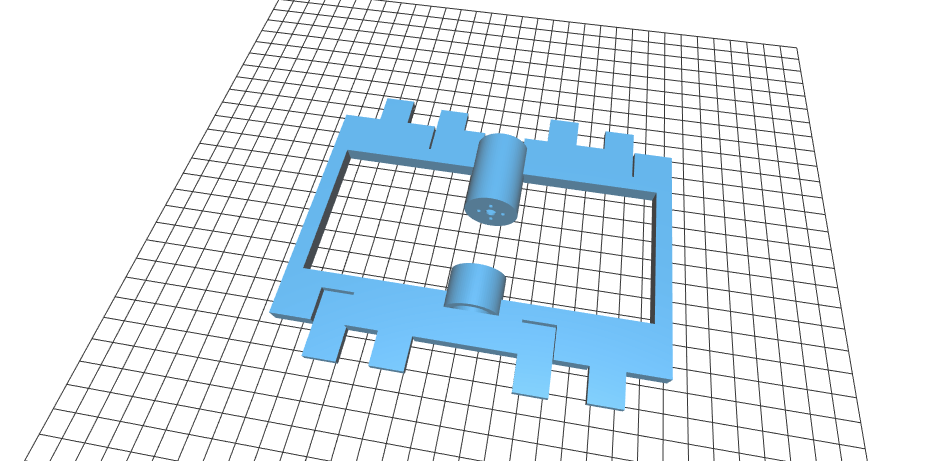
\includegraphics[width=10cm]{img/components/central_body.png}
    \caption{3D Model of the central body.}
    \label{fig: central body}
\end{figure}

\subsubsection{Lateral Body}
Used to host the wheel motor and the rest of the electronic components.
It also has lateral tabs so it can easily be joined with the central body part.
It's 3D printed and in the same orientation you see in figure
\ref{fig: lateral body}.
\begin{figure}[H]
    \centering
    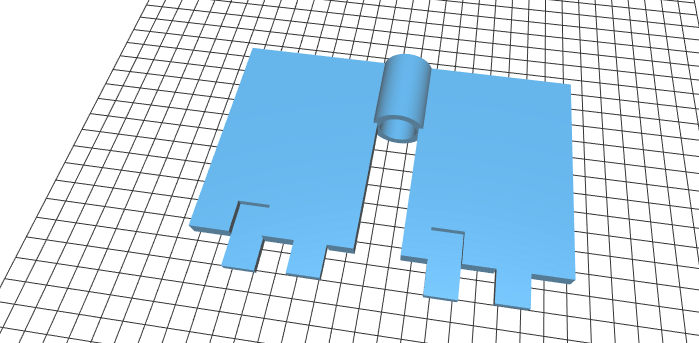
\includegraphics[width=10cm]{img/components/lateral_body.png}
    \caption{3D Model of lateral body.}
    \label{fig: lateral body}
\end{figure}
\subsubsection{Wheels}
The wheels are 3D printed. The orientation we used to print them
is putting the motor axis vertical. Each wheel is produced by two
symmetric parts that are glued together around the motor.
\begin{figure}[H]
    \centering
    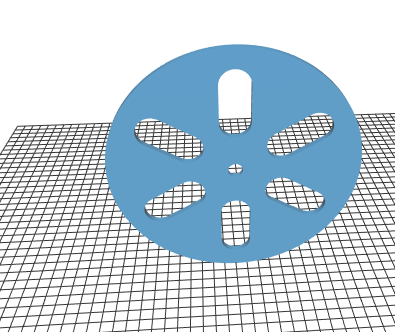
\includegraphics[width=10cm]{img/components/wheel.png}
    \caption{3D Model of a wheel.}
    \label{fig: 3D wheel}
\end{figure}
\subsubsection{Flywheel}
The flywheel is composed by 3 parts:
\begin{enumerate}
    \item 3D printed wheels very similar to the one in figure \ref{fig: 3D wheel}
    \item Steel bolts, washers and nuts.
    \item Metallic axis.
\end{enumerate}
\subsubsection{Bearings}
We are using angular balls bearing as the one seen in the figure
\ref{fig: photo bearing} to surround the flywheel axis. This bearing is
tight fit in to the 3D printed central body. The main purpose of the bearing
is to support the flywheel metal axis and help the motor with the flywheel weight
stress.
\begin{figure}[H]
    \centering
    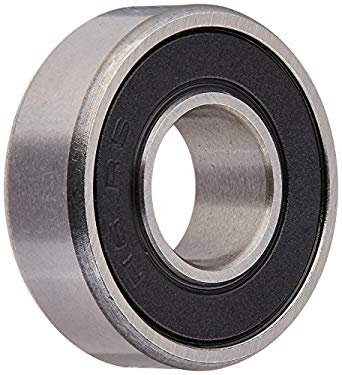
\includegraphics[width=6cm]{img/bearing.jpg}
    \caption{3D Model of a wheel.}
    \label{fig: photo bearing}
\end{figure}
\subsubsection{Reinforcements}
After we built the first prototype, we saw that the robot was suffering
from bending. So we decided to reinforce the structure with additional 3D
printed tabs and two aluminum 'U' profiles to solve the problem.

\subsection{Electronic components}
\subsubsection{Raspberry Pi}
The Raspberry Pi is a small single-board computer.
We are using Raspberry Pi 3 Model B. It has some features that we will use:
\begin{itemize}
    \item GPIO pins: General Purpose Input/Output pins are used
    \item Ethernet connection
    \item Wifi connection
    \item 5V and 3V lines
    \item DC hardware power: So we can power the Raspberry the same way as the
          other
    \item I2C: I2C is a serial protocol for two-wire interface to
          connect low-speed devices like microcontrollers. We use it to communicate
          the Raspberry Pi
\end{itemize}
\begin{figure}[H]
    \centering
    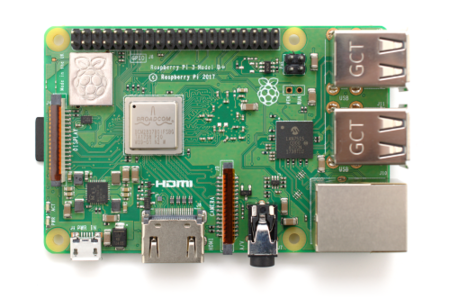
\includegraphics[width=10cm]{img/components/raspberry_pi.png}
    \caption{Raspberry Pi picture}
    \label{fig:}
\end{figure}
\begin{center}
    \begin{tabular}{ |c|c| }
        \hline
        Weight          & 42 g     \\
        \hline
        Price per unit  & 35 euros \\
        \hline
        Number of units & 1        \\
        \hline
    \end{tabular}
\end{center}
\subsubsection{Batteries}
We are using four identical batteries to power our system. They are
commercial external power supplies for smartphones. They can be recharged
via a micro-USB. We use USB cables to transmit the power to an outlet
that connects two batteries in serial that power the DC Bridges.
This bridges are powering the motors and the Raspberry.

This batteries do not work always as expected because they have
integrated security measures that disconnect them when they detect
that not power is being used.

In the other hand they incorporate many features as battery level
indicator, incorporated recharge mechanisms and on/off buttons.
\begin{center}
    \begin{tabular}{ |c|c| }
        \hline
        Weight          & 200 g    \\
        \hline
        Price per unit  & 10 euros \\
        \hline
        Number of units & 4        \\
        \hline
    \end{tabular}
\end{center}
\subsubsection{Printed Circuit Board}
In this project we tested the basic electronic with a breadboard, once we knew
the electrical components where working we decided to transfer our circuit to
a Printed Circuit Board (PCB). In particular we used a Double Sided PCB that
allows routing traces in both sides.
\begin{figure}[H]
    \centering
    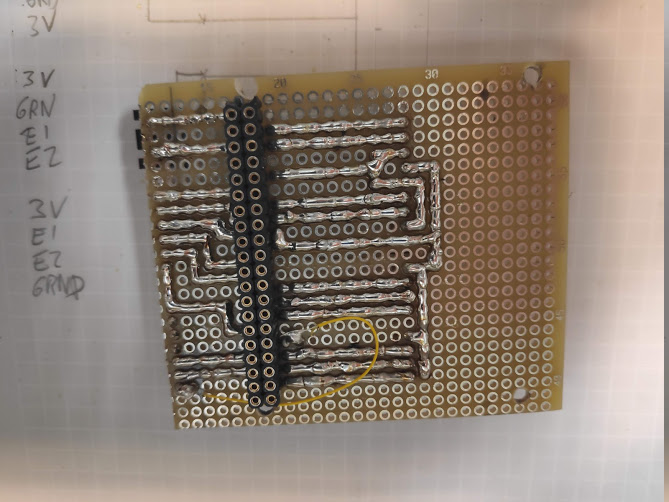
\includegraphics[width=10cm]{img/components/PCB.jpg}
    \caption{Printed circuit board}
    \label{fig: PCB}
\end{figure}

\subsubsection{DC Motor}
A DC Motor is a rotary electric machine that transforms electrical energy
(in the form of direct current) into mechanical energy through electromagnetic interactions.


Here are the specifications of our three motors:

\begin{center}
    \begin{tabular}{ |c|c| }
        \hline
        Operating voltage       & between 3 V and 9 V \\
        \hline
        Free-run speed at 6 V   & 176 RPM             \\
        \hline
        Free-run current at 6 V & 80 mA               \\
        \hline
        Stall current at 6V     & 900 mA              \\
        \hline
        Stall current at 6V     & 5 kg·cm             \\
        \hline
        Gear ratio              & 1:35                \\
        \hline
        Reductor size           & 21 mm               \\
        \hline
        Weight                  & 85 g                \\
        \hline
        Price per unit          & 10 euros            \\
        \hline
        Number of units         & 3                   \\
        \hline
    \end{tabular}
\end{center}

\begin{figure}[H]
    \centering
    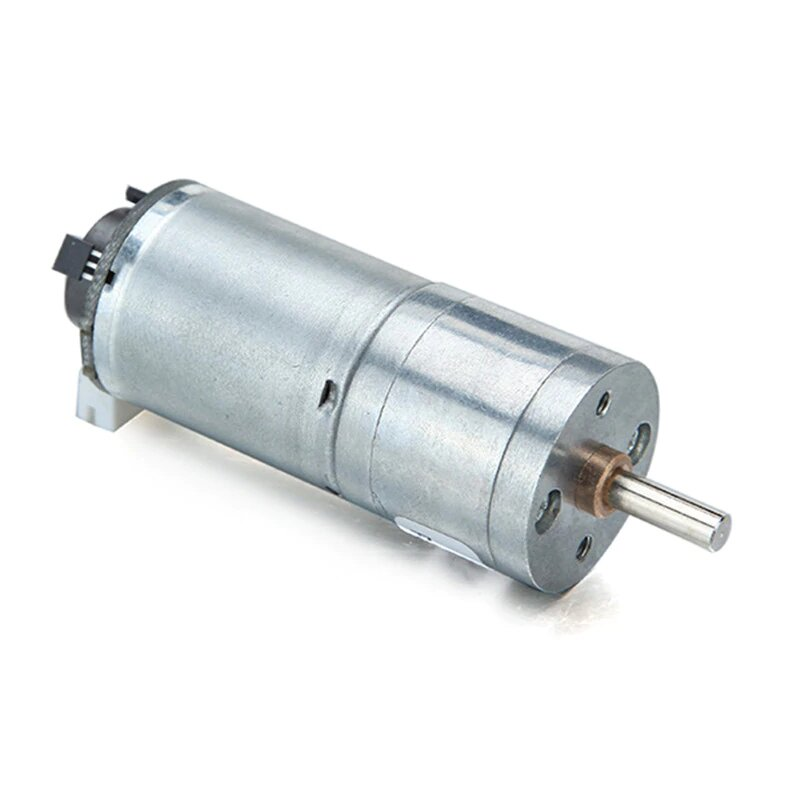
\includegraphics[width=6cm]{img/components/motor.jpg}
    \caption{DC Motor}
    \label{fig: DC Motor}
\end{figure}

\subsubsection{H Bridge}
An H bridge is an electronic circuit that switches the polarity of a
voltage applied to a load (in our case DC motors). This allows the motor to
go forwards and reverse.

Also it has the possibility to modulate the output power through a PWM signal.

Our particular H Bridge (L298N) is capable of supporting two motors at the same time.
This means that it has 6 input signals, 2 PWM (one for each motor) and 4 enable signals
(2 for each motor).

The input power for the H bridge is 10V but it has lost and it arrive to the motor
at around 8,5 V. Also it has a 5V power output that we use to feed the Raspberry
Pi.


\begin{figure}[H]
    \centering
    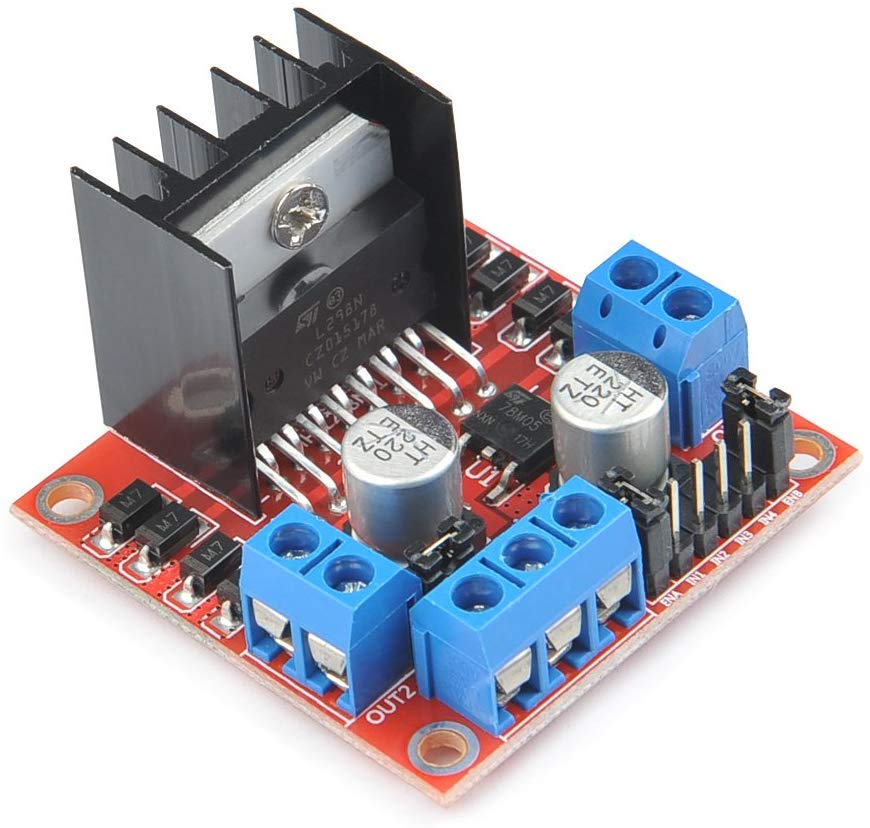
\includegraphics[width=6cm]{img/components/Hbridge.jpg}
    \caption{H Bridge}
    \label{fig: H Bridge}
\end{figure}


\subsubsection{Rotatory Encoder}
A rotary encoder, also called a shaft encoder, is an electro-mechanical device that converts the
angular position or motion of a shaft or axle to analog or digital output signals.

We programed an interruption to increment a counter to now how in what incremental position we are
and in what direction is it turning.
\subsubsection{Accelerometer}
An accelerometer is a device that measures proper acceleration. The one we are using is MPU5060.
We use the acceleration measured by the accelerometer to know in which inclination
is the platform. The accelerometer is connected to the Raspberry Pi via I2C.
